%%%%%%%%%%%%%%%%%%%%%%%%%%%%%%%%%%%%%%%%%%%%%%%%%%%%%%%%%%%%%%%%%%%%%%%%
%                                                                      %
%     File: Thesis_Versat.tex                                          %
%     Tex Master: Thesis.tex                                           %
%                                                                      %
%     Author: Andre C. Marta                                           %
%     Last modified :  2 Jul 2015                                      %
%                                                                      %
%%%%%%%%%%%%%%%%%%%%%%%%%%%%%%%%%%%%%%%%%%%%%%%%%%%%%%%%%%%%%%%%%%%%%%%%

\chapter{Simulating CPU/CGRA Architectures}
\label{chapter:simulators}

Digital circuit simulators play a fundamental role during the different phases
of circuit development, and there are multiple simulation tools that can be
used. However, despite all these tools having more or less the same purpose
(provide a way to verify the circuit), they do not work in the same way. In this
chapter a study of the state of the art of \ac{CPU} and \ac{CGRA} simulation is
done in order to understand what are the best solutions to simulate the
RV32-Versat architecture, presented in the previous chapter.

Typically, before simulating a circuit, a testbench is created. The testbench
is a program, written in a \ac{HDL} or in a programming language (like C++ or
SystemC, for example), that comprises three modules~\cite{tan:vhstas}: stimuli
generator, golden response generator and response analyser, as shown in
Figure~\ref{fig:tb}. The stimuli generator module generates the signals needed
to make the circuit work properly. The golden response generator computes the
expected circuit response, based on the inputs generated by the stimuli
generator. Finally, the response analyzer compares the circuit output signals
with the ones generated by the golden response generator. During simulation, if
both signals match, it means that the circuit is working as intended at least
for what it has been exercised for.

\begin{figure}[!htb]
	\centering
	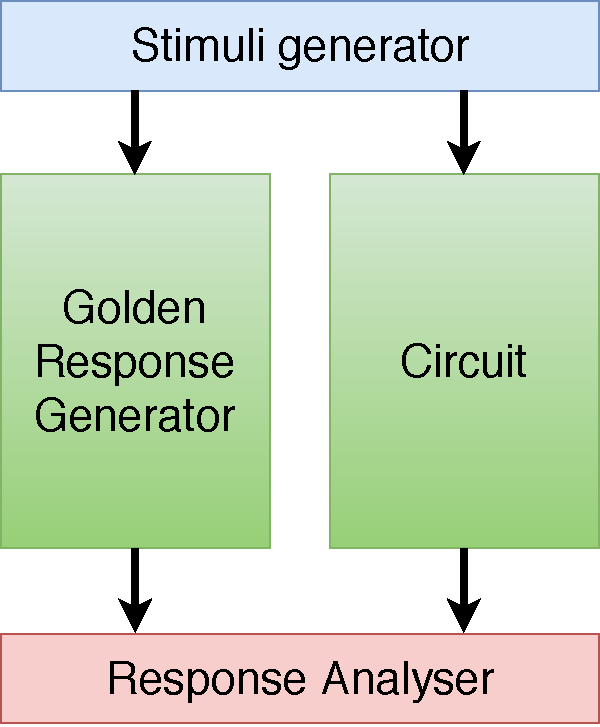
\includegraphics[width=0.42\textwidth]{Figures/Testbench.pdf}
	\caption{Testbench diagram.}
	\label{fig:tb}
\end{figure}

The results provided by the testbench might depend on the chosen simulator. This
happens because simulators work in different ways: while some focus on obtaining
the most complete results (including simulation timings), sacrificing the speed
of the simulations, others do the opposite. In this perspective, the simulators
can be divided into two main categories~\cite{tan:vhstas,palnitkar:verilog}:
event-driven or cycle-accurate.

As it will be seen in this chapter, from all the simulators studied the one that
is the most suitable to reach the objectives defined for the new simulation
environment of the RV32-Versat architecture is Verilator: it is faster than the
more traditional event-driven simulators, it is inexpensive and allows the use
of C++ and SystemC to write the testbenches, therefore simplifying the creation
of a software and hardware co-simulation environment. Also, changes in the
hardware architecture will not require changes in the simulator.

\section{Event-Driven Simulators}
\label{section:event}

The first category of simulators are the event-driven
ones~\cite{tan:vhstas,gunes:survey,palnitkar:verilog}. Most of the commercially available 
simulators belong to this category, and they work by taking events sequentially, 
propagating them through the circuit until it reaches a steady state.

The events are generated each time that a circuit input is changed, being stored
in a queue, ordered chronologically to allow the correct execution of the
events. When an event is evaluated, only the circuit nodes that have their input
changed by that event are evaluated. After evaluation, the event is removed from
the queue, with new events that result from the output changes being added to
the queue. This means that the same element might be evaluated multiple times
during the same time step due to the feedback from some signals.

It is important to mention that during the simulation process there is a timer
that is used to keep track of the events timings. This leads to one of the main
advantages of event-driven simulation, which is the accurate simulation results,
with detailed timing information, allowing the identification of timing problems
in the tested circuit.

Despite this important advantage, this type of simulation also brings some
disadvantages, mainly related with its speed. Due to their complex algorithms
used for event scheduling and timing evaluation, event-driven simulators are
slow. While for relatively small circuits this might not be a significant
problem, for large circuits this is an important disadvantage, because their
increased complexity will increase significantly the simulation duration.

Event-driven simulators are the most common type of simulators, including
simulators like the Cadence NCSim~\cite{cadence:ncsim}, the Synopsys
VCS~\cite{synopsys:vcs}, the Mentor Graphics ModelSim~\cite{mentor:modelsim} or
the free of charge open source Icarus Verilog~\cite{icarus:verilog}. Usually,
they run on a general purpose computer, being divided into three categories,
according to their algorithms: compiled-code, interpreter and gate level.

An interpreter software simulator reads the \ac{HDL} code to simulate and interprets
it, translating the original code to a set of instructions accepted by the
simulator program. This translation process occurs during runtime and implies
the creation of data structures to store the data taken from the \ac{HDL} file, that
will be used afterwards to create the simulation. These simulators are somewhat
inefficient, due to the resultant overhead of the code translation. This
typically results in the execution of a considerable number of instructions per
element evaluation, of which only a few perform logic model
evaluation~\cite{lewis:compiled}. Icarus Verilog belongs to this category: it uses a 
compiler called iverilog to compile the \ac{HDL} circuit description into the vvp 
assembly format, accepted by the simulator. After this the vvp file generated is run by 
the simulator to execute the simulation.

On the other hand, a compiled-code simulator works by transforming the \ac{HDL}
circuit description, including its testbench, into an equivalent C code (or some
similar programming language). The generated code is then compiled by a generic
complier (like gcc, for example), resulting in an executable file, that will the
be executed to run the simulation. This type of simulators are more efficient
than the interpreter ones, since they eliminate the overhead of traversing the
network data structures~\cite{lewis:compiled}. The most used simulators, like
Cadence NCSim or Synopsys VCS, belong to this category of simulators.

Although the gate level simulators are either of the interpreted or
compiled-code type, they differ from the simulators referred in those
categories~\cite{tan:vhstas}. This happens because, while those simulators have
full Verilog compliance (supporting also gate level simulations), the gate level
simulators just support a small subset of Verilog.

\ac{RTL} simulation is the most used method for circuit verification due to its
reasonable accuracy~\cite{sousa:reconfigurable}. However, in the last few years
there has been a rising trend in the industry to run gate level
simulations~\cite{khandelwal:gatelevel}. This happens mainly due to the more
complex timing checks required by modern process nodes. As a result, despite
gate level simulation being more time consuming than \ac{RTL} simulation, it greatly
improves the verification results.

\begin{figure}[!htb]
	\centering
	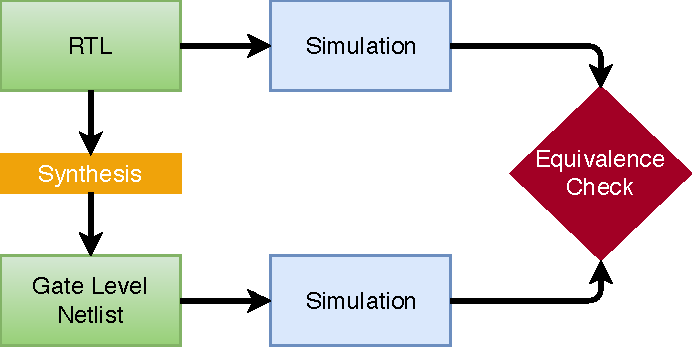
\includegraphics[width=0.7\textwidth]{Figures/Gate-level.pdf}
	\caption{Gate level design flow diagram.}
	\label{fig:gl}
\end{figure}

Usually, gate level simulation is used before going into the last stages of
circuit production. As shown in Figure~\ref{fig:gl}, the circuit is synthesized
to a gate level netlist only after the \ac{RTL} description of the circuit is
working properly. Then, the gate level netlist is simulated, with its results
being compared with the ones obtained with the \ac{RTL} description. It they are
equal, then the produced gate netlist behaves as expected, which means that no
synthesis problems have been introduced neither by the designer nor by the
synthesis tool.

\section{Cycle-Accurate Simulators}
\label{section:cycle}

Cycle-Accurate simulators are another important category of HDL
simulators. Instead of taking events sequentially, propagating them through the
circuit until it reaches a steady state, like the event-driven simulators, this
type of simulators evaluate each logic element of the circuit in a clock
cycle. They do this evaluation for each clock cycle, without taking into
consideration the propagation times and delays within the
cycle~\cite{khandelwal:gatelevel}.

As a result, these simulators are considerably faster than the event-driven
ones. However, they provide incomplete information about the circuit, since they
do not evaluate the delays and propagation times when evaluating each clock
cycle. So, if a circuit has timing problems, a cycle-accurate simulator will not
be able to notice them, making necessary the use of an event-driven simulator at
some stage to evaluate the existence of timing problems. All these
characteristics make the cycle-accurate simulators best suited for large circuit
simulation, like CPUs, when simulation speed is an important factor.

Most cycle-accurate simulators use a 2-state model (0 or 1) to calculate the
values of the signals through the circuit. A typical event-driven simulator uses
a more complex model, with more states (adding states like undefined, unknown or
high-impedance)~\cite{bennett:verilator}. This means that cycle-accurate
simulators have to make assumptions when the signals may have a value different
from 0 or 1 (for example, a signal that was uninitialized). While this speeds up
the simulation process, it also might be prone to produce wrong results.

From all the cycle-accurate simulators available, the most used one is probably
Verilator. Verilator is an open source simulator that compiles synthesizable
Verilog RTL, generating cycle accurate C++ and SystemC models. For each circuit, Verilator
compiles a different model. These models are
then linked to a testbench, being executed in order to generate the
simulation. Verilator does not only translate Verilog code to C++ or
SystemC. Instead, it compiles the code into a much faster optimized and
thread-partitioned model, which is in turn wrapped inside a C++/SystemC
module~\cite{veripool:verilator}, that can be used afterwards in a software and hardware 
co-simulation environment.

\section{Hardware-Based Simulators}
\label{subsection:hardware}

As the name indicates, hardware-based simulators are a type of simulators that
rely on configurable hardware to do the digital circuit verification. When
compared with the software-based simulators presented previously (event-driven and 
cycle-accurate), they have the advantage of being a
few orders of magnitude faster~\cite{tan:vhstas}. However they also have some
disadvantages: the hardware can be costly sometimes (depending on its
specifications) and it requires long compilation times, which makes them
needless for smaller designs. These simulators also require proprietary hardware
platforms to perform the desired simulations, with the hardware setup depending
on the platforms used, being different on each platform. As a result, these type
of simulators have a steep learning curve.

In this simulation type, the Verilog design is mapped onto a reconfigurable
piece of hardware with the same logical behaviour as the netlist.  The simulation
is divided between the software simulator, which simulates all the Verilog code
that is not synthesizable, and the hardware accelerator, which simulates
everything that is synthesizable~\cite{khandelwal:gatelevel}. The design is then
run on the hardware, producing the simulation results. The results, like in a
software-based simulator, must be checked in order to assess if the circuit is
working properly.

There are two variants of hardware-based simulators: \ac{FPGA}-based or
emulator-based. On one hand, the \ac{FPGA}-based simulators, as the name indicates,
rely on \ac{FPGA}s. A \ac{FPGA} is an integrated circuit designed to be configured 
multiple times, according to the user needs. It comprises an array of programmable logic 
blocks, memory elements, arithmetic functions, etc.

\begin{figure}[!htb]
	\centering
	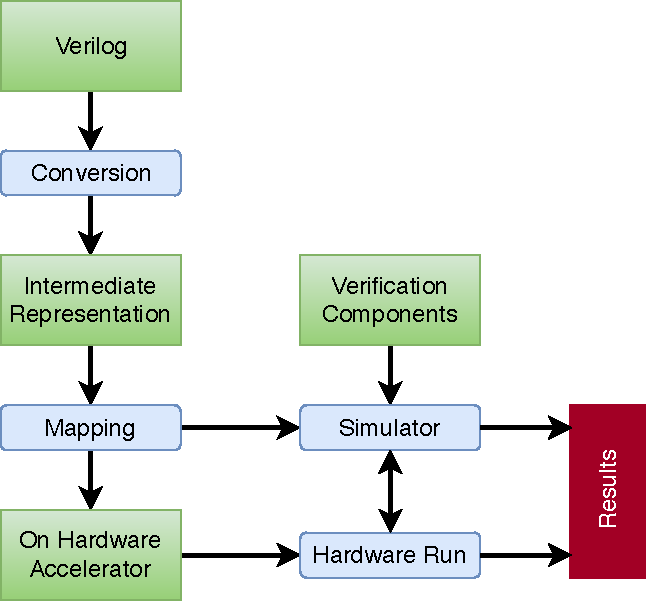
\includegraphics[width=0.7\textwidth]{Figures/FPGAsim.pdf}
	\caption{FPGA-based simulation flow~\cite{khandelwal:gatelevel}.}
	\label{fig:fpga}
\end{figure}

The \ac{FPGA}-based simulators follow the flow shown in Figure~\ref{fig:fpga}. The
original Verilog description of the code is transformed into an intermediate
representation, independent of the target platform. Here, the synthesizable
portions of the code are mapped into the \ac{FPGA}, while the non synthesizable
portions (namely intendend for verification purposes) are run as software in the
host machine (software/hardware co-simulation). The simulator and the \ac{FPGA}
interact with each other to produce the results.

On the other hand, Emulator-based simulators rely on \ac{ASIC} or \ac{FPGA}s to run their
simulations. When compared to an \ac{FPGA} an \ac{ASIC} offers limited
reconfigurability, but with the advantage of a higher simulation speed.

This type of simulation offers the possibility of testing the software before
having it implemented on chip, as the software application can run exactly as it
would on the real chip in a real system. It also offers the possibility of
testing more complex programs, that would take large amounts of time (sometimes
even days) running on other types of simulators (like the software-based ones).

The simulation flow for this type of simulators has some similarities with the
\ac{FPGA}-based simulators. In this case, as shown in Figure~\ref{fig:emulator}, the
Verilog code is converted into an intermediate representation, that will the be
mapped into the emulator. The code to be mapped must include only code that can
be implemented into the emulator. This means that the non synthesizable code
must be separated, being included in the software application. Both the software
and hardware platform interact with each other to produce the results.

\begin{figure}[!htb]
	\centering
	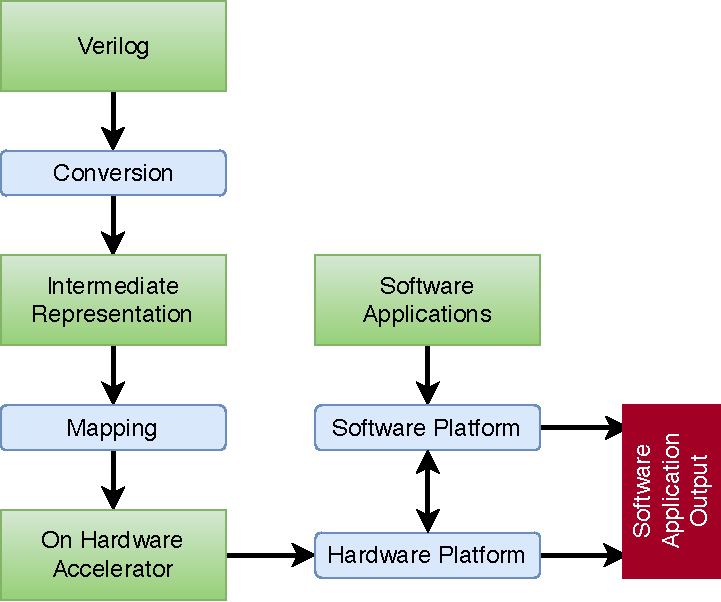
\includegraphics[width=0.7\textwidth]{Figures/Emulatorsim.pdf}
	\caption{Emulator-based simulation flow~\cite{khandelwal:gatelevel}.}
	\label{fig:emulator}
\end{figure}

\section{Performance Comparison}
\label{section:performance}

In Figure~\ref{fig:performance} a chart comparing the performance of the most
popular Verilog software-based simulators available in the 
market~\cite{verilator:benchmarks} is shown. To run these benchmarks, a slightly modified 
model of the Motorolla M68K processor is used as the design under test. All the 
simulators shown were run on a general purpose computer with an 2.2GHz AMD Phenom 9500 
processor, 667MHz DDR2 Memory and running the SuSE 11.1 operating system. The benchmark
measures the number of clock cycles that a simulator can run in a fixed amount
of time, so a higher result means that the simulator has a better performance.

\begin{figure}[!htb]
	\centering
	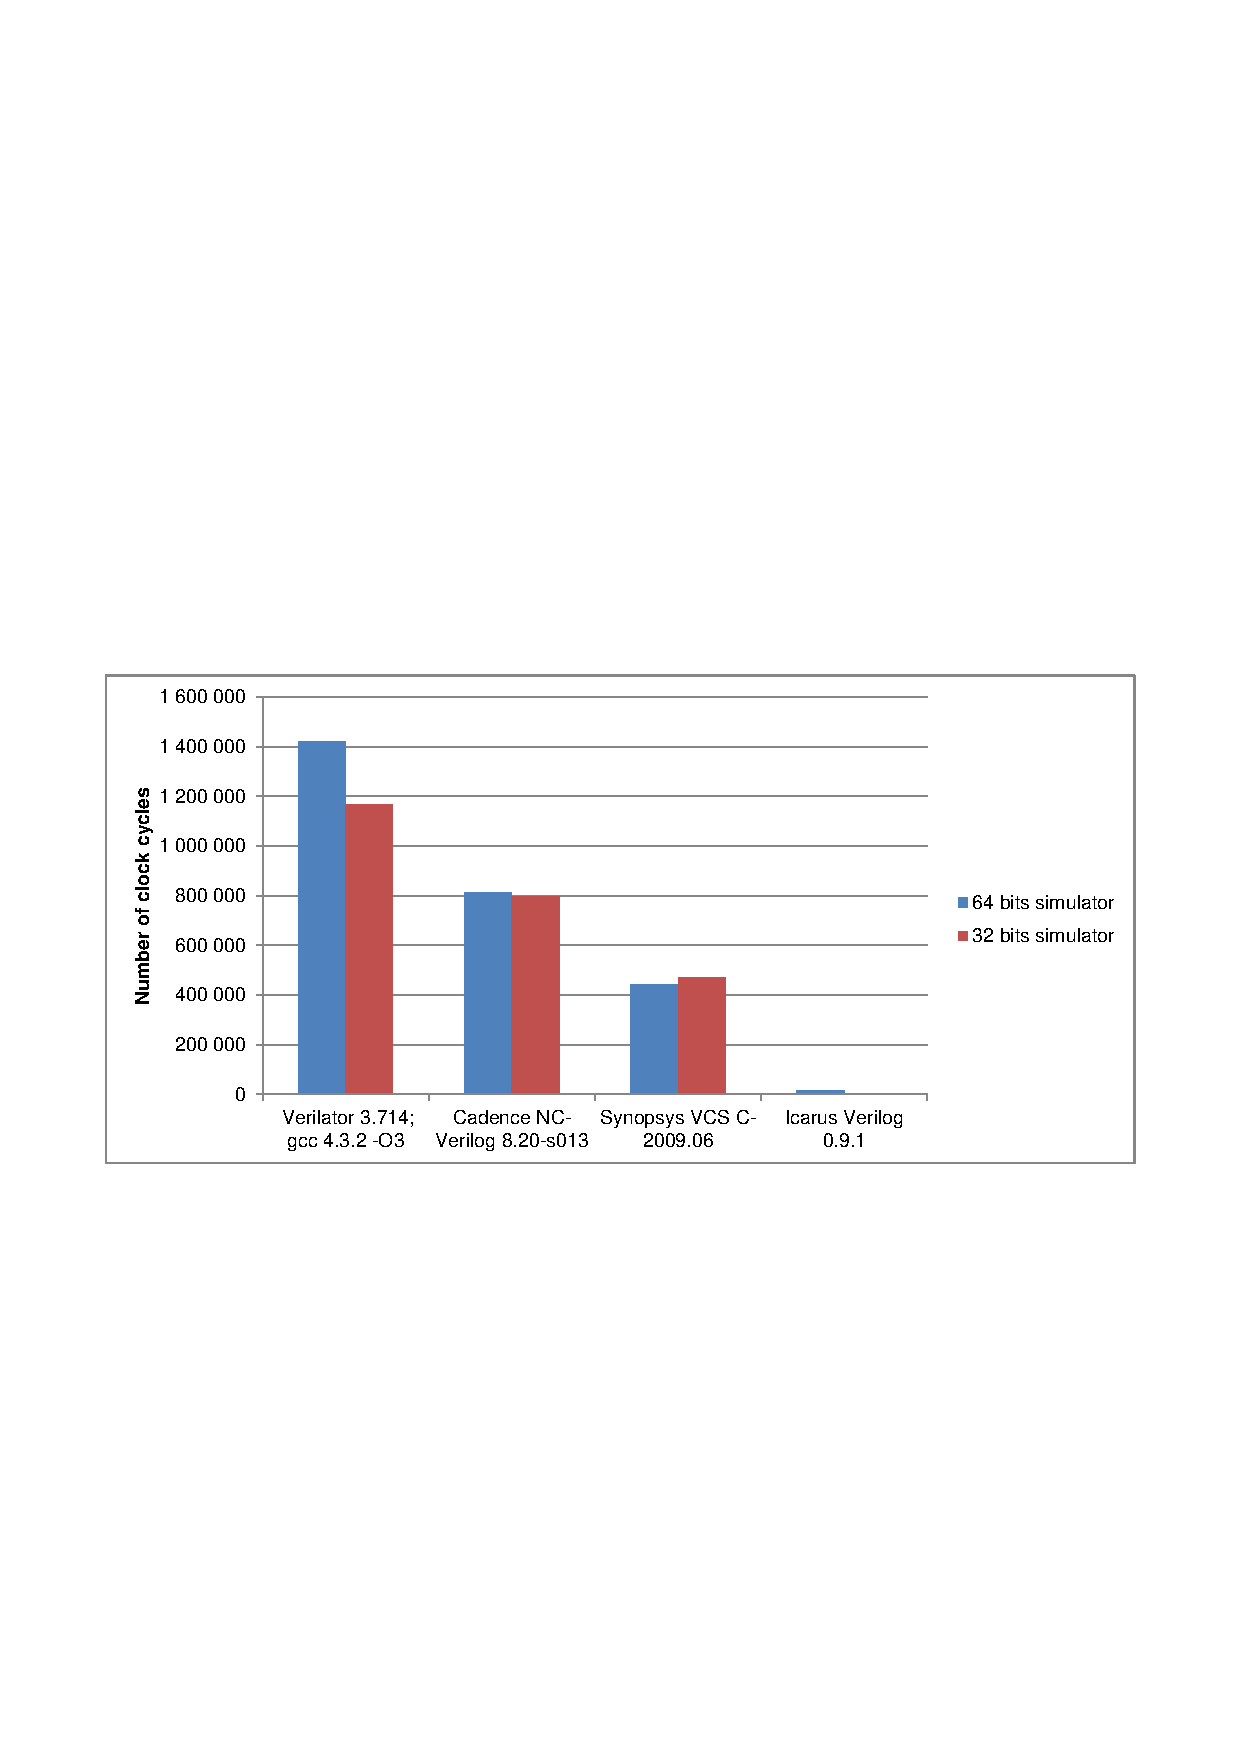
\includegraphics[trim=0 280 0 310 , clip, 
	width=0.93\textwidth]{Figures/Performance.pdf}
	\caption{Benchmark results for different Verilog 
		simulators~\cite{verilator:benchmarks}.}
	\label{fig:performance}
\end{figure}

From the analysis of the benchmark results, it can be concluded that Verilator
is considerably faster than the other tested simulators, both in 32 and 64 bits
versions. Cadence NCSim is almost 2 times slower than Verilator, while Synopsis
VCS is 3.5 times slower. Icarus Verilog is the slowest simulator tested, being
almost 80 times slower than Verilator. This result was expected if we take into
account that Verilator is a cycle-accurate simulator, while the other simulators
are event-driven. Recall that event-driven simulators have lower performance
despite offering more detailed simulations. Among the event-driven simulators,
Icarus Verilog is the slowest since it is of the interpreter type while the
others are of the compiled-code type. Therefore, Icarus has to deal with the
overhead of code translation, as explained before.

The benchmark results shown should only work as reference, given their
limitations: the versions of the simulators used are already outdated, the same
happening with the hardware and operating systems used in the general purpose
computers. Also, this benchmark only evaluates the performance in one model
(Motorolla M68K processor), instead of using multiple models in order to provide
more accurate results.

Also, the benchmark runs were made in single-threaded mode, when most commercial
simulators (including the ones analysed) support simulations in multi-threaded
mode. This consists in creating multiple threads for the different processes and
distributing them over multiple cores in a chip or even across multiple chips,
which execute in parallel. The threads are usually inter-dependent, so there
should be a synchronization process when transferring data between threads. This
process is time consuming, since different threads have different execution
times, requiring the faster threads to hold on until the slowest thread
finishes~\cite{tan:vhstas}.

Despite the concurrent nature of the Verilog statements, it is not feasible to
parallelize the totality of the statements in a model, since the number of
statements is much greater than the amount of threads available. Moreover, this
would require a great amount of synchronization between the different threads,
killing the possible speed-up. Instead, the Verilog top-level code is divided in
multiple subsystems, with each one being simulated as a different thread.

Parallelization is the solution found to achieve considerable performance
improvements in simulators. This happens because throughout the years the
algorithms used in the simulators were optimized to such a point where it became
difficult to find further optimizations. So the only viable solution was to
start using parallelization techniques.

\section{CGRA Simulation}
\label{section:CGRA}

As referred before in this work, \ac{CGRA} architectures have some big
differences when compared with dedicated circuits. This poses difficulties in
some areas, being one of these areas the simulation of the developed
architectures. Unlike a dedicated circuit, in a \ac{CGRA} the reconfigurable
interconnects between the functional units allow building a multitude of
different datapaths at run-time. This is an overhead compared to simulating the
various datapaths separately without simulating the reconfigurable
infrastructure.

As a result, simulating CGRAs with event-driven simulators will result in
lengthy simulation times. Consequently, finding a valid alternative to simulate
\ac{CGRA}s (in this particular case, the Versat architecture) could save an
important amount of time and money during the development of applications for
this type of architectures.

Using cycle-accurate simulators could be a good alternative to speed up
\ac{CGRA} simulations. As seen in the previous chapter, the use of a
cycle-accurate simulator like Verilator could considerably cut the simulation
time, reducing it, at least, by a factor of 2 (see
Fig~\ref{fig:performance}). It also has the advantage of having no additional
cost, since Verilator is open source. However, the \ac{CGRA} (or any other
circuit) should not be tested exclusively with a cycle-accurate simulator, since
their results do not take into account the propagation delays inside the
\ac{CGRA}, and also make some simplifications regarding the signal states. This
is specially true if the \ac{CGRA} is in constant development.

Another alternative is doing simulations at a high-level, instead of doing them
at the \ac{RTL} level. High-level simulation techniques have been applied in
different types of circuits, like processors, with good results. However, for
\ac{CGRA} there is an additional difficulty compared to regular processors for
this type of simulations because of the reconfiguration process. Two examples of
approaches to high-level simulation are presented next: one that proposes a
cycle-accurate simulator~\cite{chen:CGRA}, and another one that proposes a
framework for high-level simulation of \ac{CGRA}s~\cite{pasha:CGRA}. However,
both approaches have a problem: they are specifically tailored for an
architecture, so each time there is a significant change in the architecture,
the simulators will also need to be changed. With Verilator, for example, that
does not happen.


\subsection{High-Level Cycle-Accurate Simulator}
\label{subsection:hlcycle}

The high-level cycle-accurate approach that is proposed in~\cite{chen:CGRA}
introduces the concept of a timing-constrained datapath. In \ac{CGRA}s there is
not a well defined pipeline structure due to the reconfigurable
interconnects. The pipeline is formed on the fly with registers or memories
being used to save the intermediate results between the different datapaths.

With this in mind, a register-centric synthesis technique is used using a
timing-constrained datapath rooted at a chosen register. For the example in
Figure~\ref{fig:datapaths}, the datapath is rooted at the register R0, with the
different paths being tracked down within the timing constraint given. These
datapaths can finish either on a circuit input or on an intermediate register.

\begin{figure}[!htb]
	\centering
	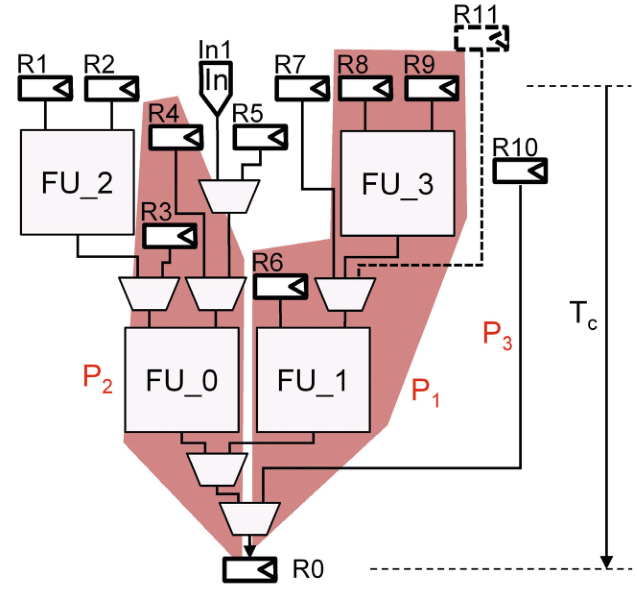
\includegraphics[width=0.6\textwidth]{Figures/Datapaths.png}
	\caption{Timing-constrained datapath example~\cite{chen:CGRA}.}
	\label{fig:datapaths}
\end{figure}

The timing-constrained datapaths will be extracted and used by the compiler,
being converted into a pattern graph of \ac{FU}s. In this way, the simulation
becomes a signal flow graph simulation, being performed via a routine that
updates the value of all registers and output ports on each clock cycle. For the
register/port udpate routine the obtained graph will be traversed, starting on
the root register, and evaluating all the possible paths. This means that the
simulator only does the necessary operations for the existent configuration
bits, and also that the worst case for the simulation execution time will be
proportional to the number of configuration bits available on the longest path
of the flow graph.

The main simulation routine uses three main components: Input Read,
Register/Port Update (described previously) and State Update. The Input Read is
responsible for reading all the inputs on each clock cycle, and the
Register/Port Update for updating all the values of registers and ports that
need to be updated.

To evaluate the performance of this simulator, multiple simulations were made,
using two different \ac{CGRA}s: \ac{CGRA}-1 (modelled similarly to ADRES
architecture~\cite{mei:reconfigurable}) and \ac{CGRA}-2 (similar
to~\cite{chen:flexdet}), and running six different application kernels (3 on
each \ac{CGRA}). The simulation speed was compared with some commercially
available simulators (Synopsys VCS-MX 2011.03 and Verilator 3.853), using a
system with an AMD Phenom II X4 955 CPU and 8 GB of memory. To run the
simulations the timing constraint was set to 3 \ac{FU}s, since the performance
of the kernels is the same as without timing constraint. Both the generated
high-level simulator and Verilator were compiled with GCC 4.4.7. The obtained
results are shown in Figure~\ref{fig:hlperformance}, normalized with the
simulation time for the high-level simulator.

\begin{figure}[!htb]
	\centering
	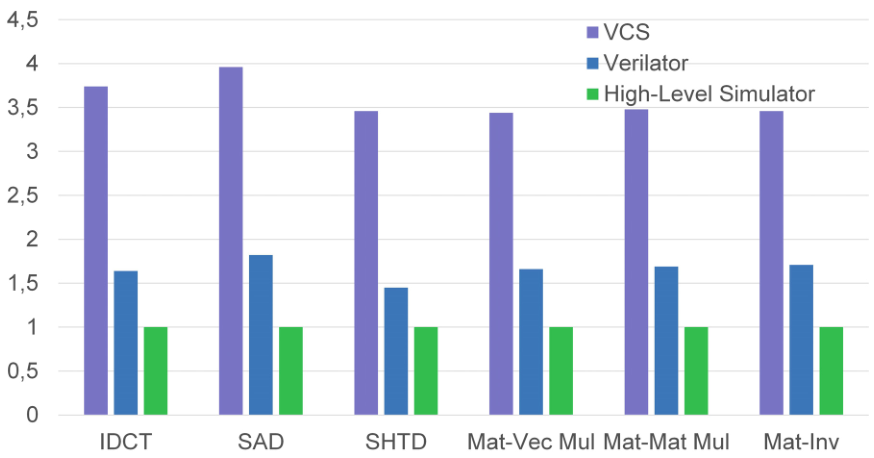
\includegraphics[width=0.8\textwidth]{Figures/hlperformance.png}
	\caption{Performance comparison between the high-level and other commercially 
		available
		simulators~\cite{chen:CGRA}.}
	\label{fig:hlperformance}
\end{figure}

From the results in Figure~\ref{fig:hlperformance} it can be seen that the
high-level simulator is almost 4 times faster than Synopsys VCS and around 1.5
times faster than Verilator. This was already expected given that, while the
high-level simulator only considers the values in the registers after each
execution cycle, the other simulators also evaluate the intermediate signals.

\subsection{CGRA High-Level Simulation Framework}
\label{subsection:framework}

The framework presented in~\cite{pasha:CGRA} provides a high-level simulation
and optimization solution for a given mesh-based \ac{CGRA}. It accepts applications
written in C, generating the corresponding VHDL description for the target \ac{CGRA},
and it can be divided into two main parts: C to netlist transformation and
netlist to \ac{CGRA} mapping.

The C to netlist transformation relies on GeCoS~\cite{l'hours:FPGA}, an
open-source compiler mainly used for \ac{ASIP} to compile the C code, generating a data 
flow graph that represents the original C code. This was made using GeCoS direct acyclic 
graphs generation capabilities. To transform the generated graphs into netlists for the 
target \ac{CGRA}, a parser was created. In the resulting netlist, each \ac{ALU} 
corresponds to a node in the original graph.

For the netlist to \ac{CGRA} mapping, the previously generated netlists are placed
into the target \ac{CGRA}, using a simulated annealing algorithm. The placement and
routing algorithms for netlist to CGRA mapping used are independent of the \ac{CGRA}
architecture, so they can be used for exploring different architectures. In the
end an estimation of the area used is calculated.

The performance of the developed framework was only compared with \ac{FPGA}
implementations. However, it would be more useful (in the scope of this thesis)
to compare how this new framework performs simulating a \ac{CGRA} when compared with
other commercial \ac{HDL} simulators, using the same architecture.
